\documentclass[journal]{IEEEtran}
\usepackage[utf8]{inputenc}
\usepackage[T1]{fontenc}
\usepackage{amsmath}
\usepackage{graphicx}
\usepackage{booktabs}
\usepackage{multirow}
\usepackage{xcolor}
\usepackage{tikz}
\usetikzlibrary{arrows.meta,positioning}
\usepackage[hidelinks]{hyperref}

\begin{document}

\title{Reimplementation and Controlled Improvement of a Machine Learning Pipeline for ECG Heartbeat Classification on MIT-BIH}

\author{Student Project Team, Course AIL303 --- Machine Learning\\
FPT University, Da Nang Campus, Vietnam}

\maketitle

\begin{abstract}
Automated electrocardiogram (ECG) analysis is central to early diagnosis and remote monitoring of cardiac arrhythmia. Subba and Chingtham (IEEE Access, 2024) reported 98\% heartbeat classification accuracy on the MIT-BIH Arrhythmia Database with wavelet denoising, handcrafted features (R-peak statistics, higher-order statistics and FFT magnitude) and a Random Forest. We first reimplement this pipeline as modular, reproducible software and measure 97.57\% accuracy, but only 69.96\% sensitivity for supraventricular ectopic beats (SVEB) and 55.63\% for fusion beats (FB). We then run five controlled experiments, each changing exactly one factor and each motivated by the previous errors, signal-processing reasoning and prior literature: RR-interval features, time-domain morphology, LightGBM instead of Random Forest, SMOTE instead of random up-sampling, and patient-normalised RR intervals. On the original protocol the best model reaches 99.42\% accuracy and 95.42\% macro-F1 (baseline 87.60\%), with SVEB sensitivity 95.14\%. Because the original random beat split mixes beats of the same patient in training and test sets, we also evaluate the standard inter-patient split. There, the baseline almost never detects SVEB (0.22\% sensitivity), while our final version reaches 61.89\% and raises macro-F1 from 33.75\% to 50.15\%. All code, notebooks and results are released.
\end{abstract}

\begin{IEEEkeywords}
Electrocardiogram (ECG), arrhythmia classification, MIT-BIH, feature extraction, RR interval, LightGBM, SMOTE, inter-patient evaluation, reproducibility.
\end{IEEEkeywords}

\section{Introduction}
\IEEEPARstart{E}{lectrocardiography} is the most widely used non-invasive technique for monitoring the electrical activity of the heart. The P, QRS and T deflections of each beat carry diagnostic information that clinicians usually read by hand, a process that is slow, subjective and hard to scale to continuous or remote monitoring. Machine learning (ML) offers automated, objective heartbeat classification, and the MIT-BIH Arrhythmia Database~\cite{moody2001} is the common benchmark.

Subba and Chingtham~\cite{subba2024} proposed a pipeline that combines wavelet denoising, baseline-wander removal, class rebalancing by up-sampling, and a handcrafted feature set (amplitude/temporal statistics, higher-order statistics and FFT features) with five classical classifiers. Random Forest (RF) was best, with 98\% accuracy over the five AAMI classes (N, SVEB, VEB, FB, Q).

This work has two parts. First, we reimplement the pipeline as modular software and document the choices the original description leaves open (Sections~\ref{sec:data}--\ref{sec:impl}). Second, we improve it through a sequence of controlled experiments in which every version changes exactly one factor relative to the previous one and states why (Section~\ref{sec:improve}). We also check how much of the result survives on unseen patients (Section~\ref{sec:inter}). Our contributions are:
\begin{itemize}
\item an open, modular reimplementation of~\cite{subba2024}, with measured (not only target) results;
\item five one-factor improvements that raise macro-F1 from 87.60\% to 95.42\% on the original protocol;
\item an inter-patient evaluation showing that the random beat split is strongly optimistic, and that patient-normalised RR features are the key change for unseen patients.
\end{itemize}

\section{Related Work}
Classical approaches pair engineered features with shallow classifiers. De Chazal et~al.~\cite{dechazal2004} combined RR-interval and morphology features with linear discriminants and introduced the inter-patient DS1/DS2 protocol. Mondéjar-Guerra et~al.~\cite{mondejar2019} fused RR, wavelet, HOS and local binary pattern features in an SVM ensemble. Lin and Yang~\cite{lin2014} showed that RR intervals normalised by each patient's average improve SVEB detection. Ensembles of RF and SVM~\cite{bhattacharyya2021} and higher-order spectra with graph Fourier features~\cite{liu2020} report 96--98\% accuracy. Optimised SVMs with particle swarm optimisation and ICA have also been studied~\cite{ramkumar2021}.

Deep learning applies convolutional and recurrent networks directly to the signal: 1-D residual CNNs~\cite{khan2023}, attention-based dual RNNs with dilated CNNs~\cite{islam2023} and multi-scale networks for 12-lead ECG~\cite{zhang2024}, often above 99\% accuracy on intra-patient splits. Luz et~al.~\cite{luz2016} survey the field and stress that intra-patient results are not comparable to inter-patient ones. For class imbalance, SMOTE~\cite{chawla2002} is the standard data-level remedy; for tabular features, gradient-boosted trees such as LightGBM~\cite{ke2017} remain very strong~\cite{grinsztajn2022}.

\section{Dataset and Problem Formulation}\label{sec:data}
MIT-BIH contains 48 half-hour two-lead recordings from 47 subjects, sampled at 360\,Hz. We use lead~0 and the expert beat annotations. The 15 MIT-BIH beat symbols are grouped into five AAMI EC57 classes with the de Chazal mapping (Table~\ref{tab:aami}). After removing beats whose 360-sample window crosses the record boundary, 109{,}438 beats remain: N 90{,}582, SVEB 2{,}781, VEB 7{,}235, FB 802, Q 8{,}038.

\begin{table}[t]
\centering
\caption{AAMI class mapping.}\label{tab:aami}
\begin{tabular}{lll}
\toprule
Class & Description & MIT-BIH symbols\\
\midrule
N & Normal beat & N, L, R, e, j\\
SVEB & Supraventricular ectopic & A, a, J, S\\
VEB & Ventricular ectopic & V, E\\
FB & Fusion & F\\
Q & Unknown / paced & /, f, Q\\
\bottomrule
\end{tabular}
\end{table}

We use two evaluation protocols.
\textbf{Random split} (the protocol of~\cite{subba2024}): a stratified 80/20 split of all beats with seed 42 (87{,}550 training and 21{,}888 test beats).
\textbf{Inter-patient split}~\cite{dechazal2004}: train on the 22 records of DS1 (50{,}995 beats) and test on the 22 different patients of DS2 (49{,}687 beats); the four paced records are excluded.
Since N makes up 83\% of the beats, accuracy mostly reflects the N class. We therefore use \emph{macro-F1} and the sensitivity (Se) of SVEB and FB as the main metrics, together with accuracy for comparison with~\cite{subba2024}.

\section{Pipeline}\label{sec:method}
Fig.~\ref{fig:pipe} shows the pipeline. The code is split into small modules (\texttt{dataset}, \texttt{preprocess}, \texttt{features}, \texttt{models}, \texttt{metrics}, \texttt{run}), and every experiment version is one entry in a configuration file.

\begin{figure}[t]
\centering
\resizebox{\columnwidth}{!}{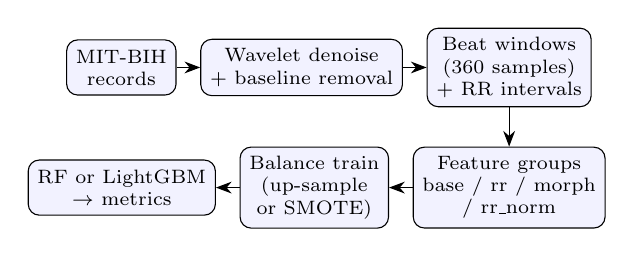
\begin{tikzpicture}[node distance=3mm, every node/.style={font=\scriptsize},
  box/.style={draw, rounded corners, align=center, minimum height=7mm, fill=blue!5},
  arr/.style={-{Stealth[length=2mm]}}]
\node[box] (a) {MIT-BIH\\records};
\node[box, right=of a] (b) {Wavelet denoise\\+ baseline removal};
\node[box, right=of b] (c) {Beat windows\\(360 samples)\\+ RR intervals};
\node[box, below=5mm of c] (d) {Feature groups\\base / rr / morph\\/ rr\_norm};
\node[box, left=of d] (e) {Balance train\\(up-sample\\or SMOTE)};
\node[box, left=of e] (f) {RF or LightGBM\\$\rightarrow$ metrics};
\draw[arr] (a) -- (b); \draw[arr] (b) -- (c); \draw[arr] (c) -- (d);
\draw[arr] (d) -- (e); \draw[arr] (e) -- (f);
\end{tikzpicture}}
\caption{Pipeline. The split into training and test sets is made before balancing, so the test set keeps its natural class distribution.}\label{fig:pipe}
\end{figure}

\subsection{Preprocessing}
Each full record is denoised with a 9-level \texttt{bior4.4} wavelet decomposition in which the lowest- and highest-frequency sub-bands are set to zero before reconstruction. Baseline wander is then estimated with two successive median filters of 71 and 215 samples (about 200\,ms and 600\,ms) and subtracted. A 360-sample window (1\,s) centred on each annotated R peak is cut out.

\subsection{Feature groups}
\textbf{base} (190 dims, from~\cite{subba2024}): number of R peaks in the window (\texttt{peakutils}, threshold 0.5, minimum distance 100), mean and standard deviation of the R-peak distances, mean, median, sum and standard deviation of R-peak amplitudes, skewness and excess kurtosis of the window, and the 181-point one-sided FFT magnitude.

\textbf{rr} (4 dims): pre-RR and post-RR intervals (s), the local mean of the previous ten RR intervals, and the ratio pre-RR / local mean, computed from the annotated R-peak positions of the record.

\textbf{morph} (72 dims): the beat waveform itself, mean-pooled from 360 to 72 points.

\textbf{rr\_norm} (3 dims): pre-RR, post-RR and local RR divided by the mean RR interval of the record.

\subsection{Classifiers and balancing}
RF follows~\cite{subba2024}: 100 trees, no depth limit, \texttt{min\_samples\_split}=2, \texttt{min\_samples\_leaf}=1, $\sqrt{d}$ features per split. LightGBM uses 600 trees, learning rate 0.05, 63 leaves, 0.8 row and column subsampling. Up-sampling draws each minority class with replacement to 20{,}000 training samples, leaving N unchanged; SMOTE (5 neighbours) synthesises samples up to the same count. Balancing is applied only to the training set.

\subsection{Metrics}
For each class, one-vs-rest counts give sensitivity $\mathrm{Se}=TP/(TP+FN)$, specificity $\mathrm{Sp}=TN/(TN+FP)$, positive predictive value $\mathrm{PPV}=TP/(TP+FP)$ and $F_1 = 2\,\mathrm{Se}\cdot\mathrm{PPV}/(\mathrm{Se}+\mathrm{PPV})$. Macro-F1 averages $F_1$ over the classes present in the test set.

\section{Implementation Notes}\label{sec:impl}
Several points are not fully specified in~\cite{subba2024}:
\begin{itemize}
\item \emph{Record-level denoising.} A 9-level wavelet decomposition needs a long signal; a single 360-sample beat supports only about five levels. We therefore denoise full records before cutting beats.
\item \emph{Kurtosis.} We use the standard form $\sum_i (x_i-\bar x)^4 / (n\sigma^4) - 3$, which includes the sample size $n$.
\item \emph{No leakage from balancing.} Up-sampling or SMOTE is applied after the split and only to the training set; duplicated minority beats in the test set would inflate the results.
\item \emph{AAMI mapping.} The mapping table in~\cite{subba2024} has small transcription errors; we use the standard de Chazal mapping.
\item \emph{Reproducibility.} All runs use seed 42 and were executed as Kaggle CPU notebooks (one per version). A full run of all versions takes about 15 minutes on four CPU cores; no GPU is needed.
\end{itemize}

\section{Baseline Results}\label{sec:base}
Table~\ref{tab:random} (row V0) and Fig.~\ref{fig:cm}(left) report our measured baseline on the random split. Accuracy is 97.57\%, close to the 98.0\% reported in~\cite{subba2024}. N, VEB and Q are recognised well, but SVEB and FB are not: 162 of 556 SVEB beats and 51 of 160 FB beats are predicted as N (Se 69.96\% and 55.63\%). This matches the weakness discussed in~\cite{subba2024}: SVEB and FB look similar to normal beats and are rare in the data.

\section{Controlled Improvements (V1--V5)}\label{sec:improve}
Each version changes exactly one factor relative to the previous one. For each change we state the problem in the previous result, the reasoning, and the supporting literature.

\textbf{V1: + RR-interval features.} \emph{Problem:} in V0, 162 SVEB beats are predicted as N. \emph{Reasoning:} an SVEB is a \emph{premature} beat whose QRS shape is almost normal; the difference is timing, a short RR interval before the beat and a pause after it. The FFT of a single window cannot represent this. \emph{Literature:} RR intervals are the most discriminative features for SVEB~\cite{dechazal2004,mondejar2019}.

\textbf{V2: + time-domain morphology.} \emph{Problem:} in V1, FB Se is still 64.38\% and 68 VEB beats are predicted as N. \emph{Reasoning:} the FFT magnitude discards phase, so it loses where the QRS and T waves are and how wide they are, which is exactly how fusion and ventricular beats differ from N. \emph{Literature:} raw and wavelet morphology samples are standard features~\cite{dechazal2004,mondejar2019}.

\textbf{V3: RF $\rightarrow$ LightGBM.} \emph{Problem:} each feature group helped, but 76 SVEB beats are still predicted as N and FB Se is 68.13\%. \emph{Reasoning:} RF averages independent deep trees; gradient boosting adds trees that correct the remaining errors, which helps rare, hard cases. \emph{Literature:} LightGBM~\cite{ke2017}; tree boosting is strong on tabular features~\cite{grinsztajn2022}.

\textbf{V4: random up-sampling $\rightarrow$ SMOTE.} \emph{Problem:} FB is the weakest class (Se 75.00\%). It has only 642 training beats, each copied about 31 times. \emph{Reasoning:} copies make the model memorise the same points; SMOTE interpolates new minority samples between neighbours, widening the minority region. \emph{Literature:}~\cite{chawla2002}; this was also the main recommendation of our earlier analysis of the baseline.

\textbf{V5: + patient-normalised RR.} \emph{Problem:} V4 reaches 99.42\% on the random split but only 42.79\% SVEB Se on unseen patients (Section~\ref{sec:inter}). \emph{Reasoning:} absolute RR depends on each person's heart rate, whereas prematurity is relative to that person's rhythm; dividing by the record's mean RR removes the heart-rate offset. \emph{Literature:}~\cite{lin2014,mondejar2019}.

\begin{table}[t]
\centering
\caption{Random (intra-patient) split, 21{,}888 test beats. Values in \%. Best in bold.}\label{tab:random}
\footnotesize\setlength{\tabcolsep}{3pt}
\begin{tabular}{llccccc}
\toprule
Ver. & Change & Acc & Macro-F1 & SVEB Se & VEB Se & FB Se\\
\midrule
V0 & baseline & 97.57 & 87.60 & 69.96 & 90.53 & 55.63\\
V1 & + RR & 98.47 & 91.23 & 80.22 & 94.61 & 64.38\\
V2 & + morphology & 99.01 & 93.10 & 85.25 & 96.68 & 68.13\\
V3 & LightGBM & 99.36 & 94.85 & 93.35 & 98.41 & 75.00\\
V4 & SMOTE & \textbf{99.42} & \textbf{95.42} & \textbf{95.14} & 98.41 & \textbf{78.75}\\
V5 & + normalised RR & 99.39 & 95.31 & 94.42 & \textbf{98.48} & \textbf{78.75}\\
\bottomrule
\end{tabular}
\end{table}

\begin{figure}[t]
\centering
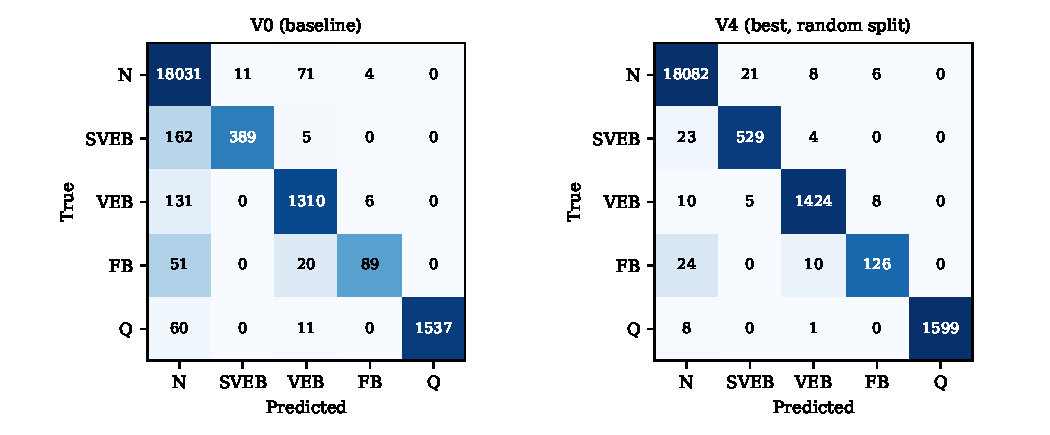
\includegraphics[width=\columnwidth]{figures/confusion.pdf}
\caption{Confusion matrices on the random split (counts; colour = row-normalised). Left: baseline V0. Right: V4.}\label{fig:cm}
\end{figure}

Table~\ref{tab:random} and Fig.~\ref{fig:prog}(a) show that every change from V0 to V4 improves macro-F1, from 87.60\% to 95.42\%, and accuracy from 97.57\% to 99.42\%, above the 98\% reported in~\cite{subba2024}. The two largest steps are the RR features (SVEB Se $+10.3$ points) and LightGBM ($+8.1$ points). SMOTE mainly helps FB ($75.00\%\rightarrow78.75\%$). Fig.~\ref{fig:cm} shows that the SVEB$\rightarrow$N errors fall from 162 to 23 and the FB$\rightarrow$N errors from 51 to 24. V5 is on par with V4 on this split, which is expected: in a random beat split the same patients are in both sets, so normalising by patient adds little.

\section{Honest Check: Inter-patient Evaluation}\label{sec:inter}
The random split places beats of the same patient, and even overlapping windows of neighbouring beats, in both training and test sets. The model can therefore recognise the patient rather than the arrhythmia, which inflates results~\cite{dechazal2004,luz2016}. We evaluate every version on the inter-patient split (Table~\ref{tab:inter}, Fig.~\ref{fig:prog}(b)).

\begin{table}[t]
\centering
\caption{Inter-patient split (train DS1, test DS2 = 22 unseen patients, 49{,}687 beats). Values in \%.}\label{tab:inter}
\footnotesize\setlength{\tabcolsep}{3pt}
\begin{tabular}{lcccccc}
\toprule
Ver. & Acc & Macro-F1 & SVEB Se & SVEB PPV & VEB Se & FB Se\\
\midrule
V0 & 90.88 & 33.75 & 0.22 & 36.36 & 84.50 & 0.00\\
V1 & \textbf{94.44} & 38.35 & 1.63 & 17.24 & 92.17 & 0.00\\
V2 & 92.66 & 36.23 & 2.29 & 22.95 & 91.30 & 0.00\\
V3 & 90.43 & 42.00 & 25.64 & 57.37 & \textbf{96.52} & 5.15\\
V4 & 90.70 & 46.27 & 42.79 & 64.74 & 95.96 & \textbf{14.69}\\
V5 & 92.29 & \textbf{50.15} & \textbf{61.89} & \textbf{71.55} & 95.84 & 14.43\\
\bottomrule
\end{tabular}
\end{table}

\begin{figure*}[t]
\centering
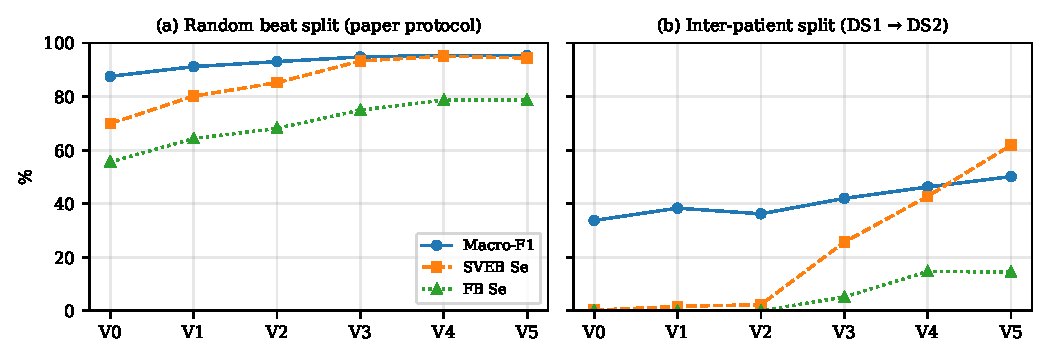
\includegraphics[width=0.85\textwidth]{figures/progression.pdf}
\caption{Macro-F1 and minority-class sensitivity per version. (a) Random split: steady gains up to V4. (b) Inter-patient split: much lower values; V5 (patient-normalised RR) gives the largest SVEB gain.}\label{fig:prog}
\end{figure*}

On unseen patients the baseline almost never detects SVEB (Se 0.22\%) or FB (0\%), although its accuracy still looks high (90.88\%) because most beats are N. The improvements largely carry over: macro-F1 rises from 33.75\% (V0) to 50.15\% (V5) and SVEB Se from 0.22\% to 61.89\%. Patient-normalised RR (V5) is the most useful change here (SVEB Se $42.79\%\rightarrow61.89\%$), although it was neutral on the random split. One change does not transfer: raw morphology (V2) lowers macro-F1 from 38.35\% to 36.23\%, because waveform shape is partly patient-specific. FB remains hard for all versions, and the Q class has only 7 test beats in DS2, which lowers macro-F1. These numbers are in the range of classical inter-patient methods, but below the best published ones~\cite{mondejar2019}.

\section{Comparison with Other Work}
On the random split, our best model (99.42\%) is above the 98\% of~\cite{subba2024} and in line with RF+SVM ensembles~\cite{bhattacharyya2021} and spectral methods~\cite{liu2020} (96--98\%), and close to deep models reporting above 99\%~\cite{islam2023,khan2023}, while training in a few minutes on a CPU. We stress that such intra-patient numbers are not comparable with inter-patient results~\cite{luz2016}; on the inter-patient split the gap to clinical use is still large, especially for FB.

\section{Conclusion and Future Work}
We reimplemented the ECG pipeline of Subba and Chingtham as modular, reproducible software and measured 97.57\% accuracy. Five controlled, one-factor changes (RR intervals, time-domain morphology, LightGBM, SMOTE and patient-normalised RR) raised accuracy to 99.42\% and macro-F1 from 87.60\% to 95.42\% on the original protocol. On the stricter inter-patient split, macro-F1 improved from 33.75\% to 50.15\% and SVEB sensitivity from 0.22\% to 61.89\%, showing that the gains are not only due to patient overlap, while also showing how optimistic the random split is. We recommend reporting the inter-patient protocol alongside the random split.

Future work includes 1-D CNNs on the raw beat combined with normalised RR features to improve FB, cost-sensitive learning and hybrid resampling (SMOTE-Tomek, SMOTE-ENN), and deployment on low-cost real-time acquisition hardware~\cite{faruk2021}.

\bibliographystyle{IEEEtran}
\bibliography{refs}

\end{document}
